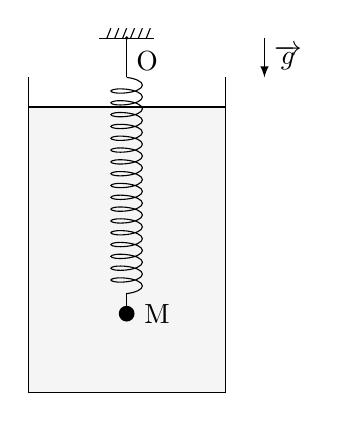
\begin{tikzpicture}[scale=.5]
\def\ptO{$O$}
\def\ptM{$M$}
\fill[gray!8!white] (0,7.25) rectangle (5,0);

\draw (0,8) -- (0,0) -- (5,0) -- (5,8);
\draw (0,7.25) -- (5,7.25);
\draw (1.8,9) -- (3.2,9);
\foreach \x in {0,.2,...,1}
{\draw (2+\x,9) -- (2.1+\x,9.25);}


\draw[decoration={aspect=0.3, segment length=1.5mm, amplitude=2mm,coil},decorate] (2.5,8) -- (2.5,2.5);
\draw (2.5,9) -- (2.5,8);
\draw (2.5,2.5) -- (2.5,2);
\fill (2.5,2) circle(.2) node at (2.7,2) [right]{$\ptM$};
\draw[-latex] (6,9) -- (6,8) node[right,midway]{$\overrightarrow{g}$};
\fill (2.5,9) circle(.05) node at (2.5,8.9) [below right]{$\ptO$};


\end{tikzpicture}